\clearpage
\section{Conclusion}\label{chap:conclusion}

There is inevitably some repetition here of the achievements of this thesis, as summarised in the \hyperlink{abstract}{Abstract} and \autoref{ch:intro}. However, additional clarity is now provided on how these achievements have been met, the value of them, and possible extensions. This value builds upon that covered in the \hyperlink{prologue}{Prologue}, primarily relating to personal motivating experiences and specific, albeit very popular, models. After this clarification, some future directions for research are presented. These range from theoretical generalisations of the new ODE well-posedness results obtained in \autoref{chap:wellposed}, to practical implications of the interval-valued excursion price processes emerging, for the first time in mathematical finance, in \autoref{chap:framework}.

\vspace{3mm}\textbf{The Heston-NIG relationship.} The priority has certainly remained to develop the mathematical theory required to describe how the classical Heston and NIG models are related in the `fast-reversion' limit of \cite{mechkov_2015}, extending the fixed-time distributive result obtained there, presented here in \autoref{thm:mech_pro}. As set out in the \hyperlink{prologue}{Prologue}, the description had to be sufficiently rich to reveal the class of derivatives whose values converge in this limit, thereby clarifying the applicability and value to practitioners depending on these models.

The extent of this relationship is now captured by the finite-dimensional limiting result of \autoref{cor:heston_fd}. This indeed reveals a wide class of derivatives with converging prices, namely those depending on the underlying price process \emph{only} through a finite number of fixed time points, sometimes called Bermudan options. But, motivated primarily by generalisations, the novel probability-free and ODE-based approach taken towards these limits in \autoref{chap:solutions} has enabled the stronger, and more informative, Hausdorff limiting result of \autoref{cor:heston_hausdorff}.

This Hausdorff result provides a complete description of the Heston-NIG relationship although, surprisingly, required the introduction of an interval-valued \emph{generalisation} of the classical NIG process. This result is ideal for practical purposes because it not only clarifies the class of continuously-monitored path-dependent derivatives whose prices \emph{will not} converge to those from the classical NIG limit, but also what these prices \emph{will} converge to.

This particular result should also be of theoretical value to anyone interested in stochastic process limit theorems, in finance or otherwise. In finance, it is the first case of an interval-valued process, like those defined and studied in the context of queuing theory in \cite{whitt_2002}, emerging. In mathematics more generally, it is the first known example of such a process arising naturally from \emph{continuous} processes through a limit of parameters. This is made all the more surprising given we are not talking about niche continuous processes, but one of the simplest and most popular stochastic volatility models. This is evidenced by \cite{heston_1993} having 10,000 citations and perhaps more importantly its implementation in numerous financial institutions and commercially available libraries like Numerix.

Over the course of \autoref{sec:price_limits} it was additionally exposed that these Heston-NIG relationships are rooted in a deeper connection between the integrated CIR and IG processes. This connection was established on the new exit-time metric space introduced in \autoref{chap:solutions}, which is stronger than Skorokhod's $\uM_1$ space. It is also easier to understand, given that it does not depend on taking infima over parametric representations, and is homeomorphic to the Polish topology of uniform convergence over compacts on the non-decreasing continuous paths. The \hyperlink{epilogue}{Epilogue} collects several other L\'evy process limits arising from the CIR process under other Heston parameterisations, e.g.~those from \cite{heston_1993} and \cite{fouque_2011}.

It is finally worth clarifying that there are immediate multi-dimensional generalisations of these limiting relationships. For example, taking a $d$-dimensional Heston model with a common CIR variance process, an analogous $d$-dimensional exp-NIG L\'evy limit is obtained with a common IG subordinator. This harmoniously connects the popular Heston FX modelling framework of \cite{decol_2013} with a less analytically and computationally demanding NIG counterpart, of growing importance as the dimension is raised. In fact this NIG counterpart falls into the tractable FX framework of \cite{ballotta_2017} built from L\'evy processes, and an implementation is available at \href{https://github.com/rmcrkd/frh-fx}{github.com/rmcrkd/frh-fx}.

\vspace{3mm}\textbf{The wider modelling framework.} All of these classical stochastic process relationships of course originate from the general limiting results for ODE solutions in \autoref{chap:solutions}, most notably \autoref{thm:exit_limit} and \autoref{cor:graph_hausdorff}. These results enabled the fractional generalisations of the Heston-NIG relationship in \autoref{sec:price_limits}, relating to the RLH model from \autoref{sec:RLH_model}.

More generally the RLH model \emph{exemplifies} the general random ODE-based framework from \autoref{sec:base_frame}, existing in both of the sub-frameworks defined in \autoref{sec:heston_frame} and \autoref{sec:martingale}. The route to \autoref{cor:RLH_martingality} brings together several results in these sections. Practically, this result establishes that the RLH price process is a martingale for all parameter combinations, so always generates arbitrage-free derivatives prices. Theoretically, it demonstrates the more general martingale result of  \autoref{thm:price_martingale}, which constitutes a novel applications of time-changes and Novikov's martingale condition to random ODE solutions. In turn, necessary integrability requirements depend on the general MGF existence result of \autoref{cor:gauss_heston_mgf}, applicable to a class of generalised Heston models with alternative Gaussian drivers.

Through the recipe in \autoref{def:rlh_polygon} and accompanying \autoref{thm:rlh_convergence} we have demonstrated how such a model can be simulated for this purpose of derivative pricing, and have provided volatility surfaces exhibiting properties associated with promising rough volatility models. So despite the RLH model being defined primarily for illustrative theoretical purposes, this all suggests that a deeper empirical comparison with leading counterparts, such as those of \cite{bayer_2016} and \cite{eleuch_2019a}, will be worthwhile.

Moving further backwards through the thesis, all models in the framework of \autoref{chap:framework} possess the well-posedness properties from \autoref{chap:wellposed}, perhaps most valuably the uniqueness and continuous dependence robustness captured by \autoref{thm:global_uniqueness} and \autoref{thm:continuity_solution_map}. These ODE results are other firsts, not depending on any spatial regularity properties of the driving functions, such as H\"older regularity, yet still being applicable to maximal solutions. Hence the description of these ODEs throughout as spatially irregular, and their resulting ability to harmoniously accommodate rough volatility models without need for additional well-posedness analysis. This starkly contrasts the ongoing line of theoretical research which aims to accommodate rough volatility within a framework of It\^o-type Volterra integral equations, e.g.~recently studied in \cite{keller-ressel_2018} and \cite{abijaber_2019c}.

Practically, this robustness means practitioners will not find that (suitably moderate) adjustments to models lead to counterintuitive consequences, e.g.~on resulting derivative prices. Accordingly, they can safely take advantage of the wide class of models captured by the solution space in \autoref{chap:solutions}, with a relatively low barrier to entry from the outset, given there is strictly no requirement to understand any form of stochastic calculus. Notice that It\^o calculus is introduced sparingly throughout this thesis, and only ever to clarify motivations from, connections with and consequences for other more familiar frameworks.

Of course more research is required until we can fully understand whether our framework built around random ODEs can take centre stage in practice, or whether its primary value will derive from what it can teach us about other frameworks. What we have already is certainly a promising start, having gone all the way from the probability-free well-posedness foundations of \autoref{chap:wellposed} to a specific model in \autoref{chap:framework} which by itself reconciles a popular classical model with rough, discontinuous and even novel excursionary generalisations.

Finally three directions for future research are provided, which this thesis has made possible.

\vspace{3mm}\textbf{Carath\'eodory ODE extensions.} The discussion leading up to the subset $\uF\subset\uC(\RR^2,\RR)$ of functions from \autoref{def:driving_func} clarifies our main motivation for considering these, given their emergence from the Heston volatility model thus potential for (practical) modelling applications. But, before our maximal uniqueness result of \autoref{thm:global_uniqueness}, we also discussed how this set $\uF$ is (theoretically) related to that in Wend's local uniqueness result in \autoref{thm:wend_uniqueness}.

Our statement of Wend's theorem is actually a reduced one, applicable only to classical \emph{differentiable} solutions, like the entirety of this thesis and majority of ODE theory. Consulting Theorem 2.6.1 of \cite{agarwal_1993}, Wend's uniqueness theorem actually holds in the extended setting where functions $f$ are not necessarily in $\uC(\RR^2,\RR)$, but satisfy the weaker `Carath\'eodory' conditions from the existence theorem of \cite{caratheodory_1927}.

Following Section 2.1 of \cite{coddington_1955} or \cite{agarwal_1993}, the Carath\'eodory conditions require each $f(\cdot,x)$ to be \emph{only} measurable, each $f(t,\cdot)$ continuous, and for each compact rectangle $\cX\subset\RR^2$ that there exists a Lebesgue integrable function $m=m_\cX$ such that $|f(t,x)|\le m(t)$ whenever $(t,x)\in\cX$. For any $(\tau,\xi)\in\RR^2$, Carath\'eodory's theorem then provides the existence of an `extended' solution $\vp$ of the ODE $x'=f(t,x)$ over some $(\tau-\ep,\tau+\ep)$ with $\vp(\tau)=\xi$. Given $f(\cdot,x)$ may not be continuous, we define such an extended solution to be absolutely continuous with $\vp'(t)=f(t,\vp(t))$ a.e.~only. The fact that Wend's theorem still holds in this setting ensures a \emph{unique} extended solution over $[\tau,\tau+\ep)$, i.e.~going forwards in time, provided $f(\cdot,x)$ is non-decreasing and $f(t,x)>0$.

Theoretically, it is natural to ask if the functions in $\uF$ can also be relaxed from $f(\cdot,x)$ being continuous to only measurable (other assumptions being equal), without compromising the maximal uniqueness of \autoref{thm:global_uniqueness}. In the generalised Heston framework in \autoref{def:gen_heston_frame}, in which our cumulative variance processes $X$ verify a random ODE of type~
\begin{equation}\label{eq:gen_hest_conc}
    X'_t = \sigma Z_{X_t} + \kappa(\vt(t) - X_t) + v,
\end{equation}
this would allow us to relax the continuity of $\vt$ to e.g.~only right-continuity. This relaxation is however not well-motivated. On the contrary, relaxing the continuous process $Z$ in \autoref{eq:gen_hest_conc} to being only right-continuous would allow us to make use of non-Gaussian L\'evy processes to drive our random ODEs $x'=Y_{t,x}$ thus cumulative variance \emph{extended} solutions $X$. This would provide an alternative to the approach from \cite{barndorff-nielsen_2001b}, applied in \cite{carr_2003}, which instead utilises SDEs driven by non-Gaussian L\'evy processes to obtain cumulative variance processes with dependent, e.g.~reversionary, increments. The L\'evy process $Z$ in these SDEs must have positive increments to ensure that $X$ does, but it is plausible that this could be relaxed in the random ODE of \autoref{eq:gen_hest_conc}.

\vspace{2mm}The main point of this extension to Carath\'eodory ODEs is \emph{not} to widen the set $\Phi$ of possible cumulative variance paths from \autoref{def:solutionset}, since we have already shown in \autoref{cor:construct_limit} how any path in the superset $\bPhi\supset\Phi$ from \autoref{def:setE} can be accommodated as a limit. Rather, we could leverage the \emph{probabilistic} properties of L\'evy processes for analytical and simulation purposes. For example, if in \autoref{eq:gen_hest_conc} $Z$ a L\'evy process, then we can consider optional sampling theory for the evaluation of $\EE[Z_{X_t}]$, thus $\EE[X_t]$, which is e.g.~not possible in the RLH model from \autoref{def:RLH_model} where $Z=W^\alpha$ is a Brownian fractional derivative.

Contrasting the usual Carath\'eodory conditions in which $f(\cdot,x)$ is measurable, e.g.~c\`adl\`ag, and $f(t,\cdot)$ continuous, this motivates the consideration of ODEs depending on the following superset $\uFe\supset\uF$. Note that while paths of L\'evy processes are not necessarily c\`adl\`ag a.s., the stochastic continuity of these processes ensure a `c\`adl\`ag modification', see e.g.~Lemma 1.4.8 in \cite{applebaum_2009}, meaning that we essentially do not lose generality by assuming this.

\begin{definition}[Set $\uFe$ of functions]\label{def:ext_driving_func}
    Let the set $\uFe$ contain functions $f:\RR^2\to\RR$ with each $f(\cdot,x)$ strictly increasing and continuous, each $f(t,\cdot)$ c\`adl\`ag with \emph{upwards} discontinuities only, so that $f(t,x)-f(t,x_-)\ge0$ for all $(t,x)$, and finally $f(\tau,\xi)>0$ for some $(\tau,\xi)\in\RR^2$.
\end{definition}

It is important to note we are \emph{not} assuming the usual Carath\'eodory conditions in \autoref{def:ext_driving_func}, but rather new ones which clearly represent an inversion of space and time. Like in \cite{barndorff-nielsen_2001b}, we assume only upwards discontinuities for now because it is easy to construct IVPs $x'=f(t,x)$, $x(0)=0$ with no maximal extended solutions otherwise, e.g.~of type $f(t,x)=t+z(x)$ in \autoref{fig:caratheodory}. That is, no solution if we do not modify the meaning of an extended solution for our inverted conditions, e.g.~to a path $\vp$ such that the exit-time $E(\vp)$ solves the inverted IVP $x'=1/f(x,t)$, $x(0)=0$ a.e., or more practically a path $\vp$ which forward Euler polygons converge to uniformly over compacts.

\begin{figure}[ht]
    \centering
    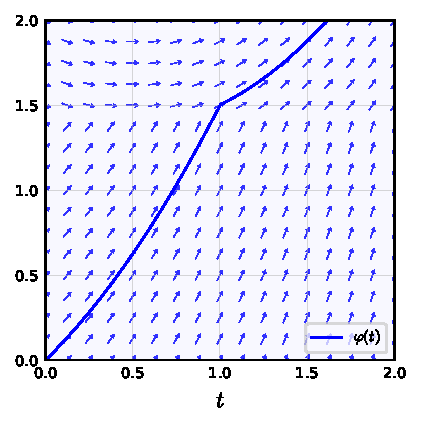
\includegraphics[width=0.48\linewidth]{figures/caratheodory1}
    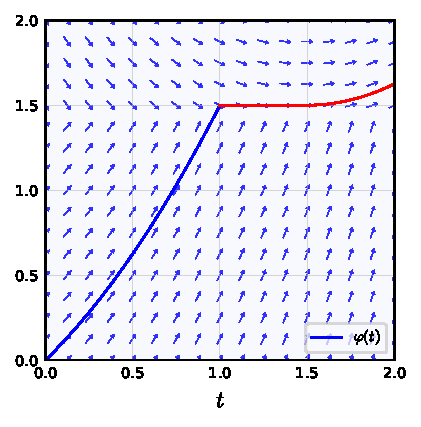
\includegraphics[width=0.48\linewidth]{figures/caratheodory2}
    \caption{Carath\'eodory extended solutions $\vp$ are shown for the IVP $x'=f(t,x)$, $x(0)=0$, where $f(t,x)=t+z(x)$ and the c\`adl\`ag path $z$ jumps \emph{downwards} at $x=1.5$. If this jump is too large, $\vp$ exists over $[0,1]$ only (right panel), although an a.e.~differentiable uniform limit of forward Euler polygons (red) may still exist.}
    \label{fig:caratheodory}
\end{figure}

Supplementing \autoref{fig:caratheodory} and \cite{barndorff-nielsen_2001b}, note that constraints on the downwards jumps of a c\`adl\`ag path peculiarly arise elsewhere, e.g.~the pathwise quadratic variation defined in \cite{lochowski_2018}. But for now we consider this coincidental.

The first and most important question towards a non-Gaussian L\'evy-driven random ODE framework is the counterpart to \autoref{thm:global_uniqueness}: are the assumptions $f\in\uFe$ and $f(\tau,\xi)>0$ sufficient for the IVP $x'=f(t,x)$, $x(\tau)=\xi$ to have a unique maximal extended solution?

\vspace{3mm}\textbf{It\^o SDE implications.} The route outlined in \autoref{ch:intro}, from the Heston volatility model in \autoref{eq:heston_intro} to the ODE in \autoref{eq:cir_ivp_well_posed}, is succinctly described by the following arrow
\begin{equation}\label{eq:route_summary}
    \dd V_t = \sigma\sqrt{V_t}\dd W^1_t + \kappa(\theta - V_t)\dd t,\ V_0=v\quad \rightsquigarrow\quad \vp'(t) = \sigma (w\circ\vp)(t) + \kappa(\theta t - \vp(t)) + v.
\end{equation}
The ODE here may be considered a pathwise counterpart of the SDE, with the correspondence $\vp'(t)=V_t(\omega)$, provided we recall that the path $w\in\uC_0(\RR,\RR)$ should not be considered one of $W^1$ but rather the time-changed version $B^1$ from \autoref{eq:tce} or later \autoref{thm:heston_ode}.

Using \autoref{thm:global_uniqueness} we now know that the corresponding IVP $x'=f(t,x)$, $x(0)=0$ has a unique maximal solution $\vp$ when $\sigma,\kappa,\theta,v>0$, for \emph{any} $w\in\uC_0(\RR,\RR)$. So uniqueness holds for the IVP even if the H\"older regularity of $w$ is taken to be far lower than that of Brownian motion, which is a.s.~$\frac12-\ep$ for every $\ep>0$. So it is natural to ask if \autoref{thm:global_uniqueness} can be utilised to establish the pathwise uniqueness of certain SDEs beyond the result of \cite{yamada_1971}, for which the CIR SDE in \autoref{eq:route_summary} is a well-known boundary case.

This question remains unanswered, even for a simple generalisation of the CIR SDE, say to $\dd V_t = \sigma |V_t|^\alpha\dd W^1_t + \theta\dd t$, $V_0=v$ for some $\alpha\in(0,\frac12)$. There is a partial answer in this case, because when $\theta=0$ this is `Girsanov's SDE', for which pathwise uniqueness fails for $\alpha\in(0,\frac12)$, see Example 1.22 in \cite{cherny_2005}. But the inclusion of a drift $\theta \dd t$ should not be underestimated, and indeed is what leads to the strictly increasing component $\theta t$ in the ODE of \autoref{eq:route_summary}, important in our proof of \autoref{thm:global_uniqueness}. Popular texts on SDEs display some neglect for such \emph{simple} drifts, because more complicated ones can often be removed by a change of measure, see e.g.~Theorem 5.27.1 in \cite{rogers_2000}.

The point now is that our new ODE uniqueness result renders this debate somewhat moot, and we demonstrate why with a practical example. Suppose we consider replacing $V_t$ on the r.h.s.~in \autoref{eq:route_summary} with $|V_t|^{2\alpha}$ for some $\alpha\in(0,\frac12)$, which is a natural consideration for a practitioner who has found the Heston model to behave undesirably, compared with their short-time observations. For some $\sigma,\kappa,\theta,v>0$, the SDE under consideration is therefore
\begin{equation}\label{eq:consider_sde}
    \dd V_t = \sigma|V_t|^\alpha\dd W^1_t + \kappa(\theta - |V_t|^{2\alpha})\dd t,\quad V_0=v.
\end{equation}
A classical result of Skorokhod's guarantees a weak solution of this SDE, see \cite{skorokhod_1965} or preferably Proposition 1.13 in \cite{cherny_2005}, the terminology of which we follow here. But this SDE need not have a \emph{unique} weak solution, let alone a unique \emph{strong} solution, i.e.~need not exhibit pathwise uniqueness. See Figure 1.1 in \cite{cherny_2005} for a succinct reminder of how these properties of SDEs are related. So probabilistic analysis of this SDE is dubious, the applicability for volatility unclear given $V$ may not be non-negative, and the convergence of simulation schemes not guaranteed. Nevertheless, \emph{given} a weak solution $(V,W^1)$, we find, just like \autoref{eq:tce}, $V$ verifies
\begin{equation}\label{eq:new_tce}
    V_t = \sigma B^1_{\int_0^t|V_s|^{2\alpha}\dd s} + \kappa\left(\theta t  - \int_0^t|V_s|^{2\alpha}\dd s\right) + v.
\end{equation}

Now let $f(t,x):=\sigma w(x) + \kappa(\theta t - x) + v$ be the usual Heston function implicit in \autoref{eq:route_summary} and consider the IVP $x'=f_\alpha(t,x)$, $x(0)=0$ with $f_\alpha\in\uF$ defined by $f_\alpha := \sgn(f)|f|^{2\alpha}$. This IVP is an example of \autoref{prob:ivp}, so by \autoref{thm:global_uniqueness} has a unique maximal solution $\vp_\alpha$ which is strictly increasing. Contrasting the solution $\vp$ in \autoref{eq:route_summary}, $\vp_\alpha$ now verifies
\begin{equation}
    \vp'_\alpha(t) = f_\alpha(t,\vp_\alpha(t)) = |f(t,\vp_\alpha(t))|^{2\alpha} = |\sigma (w\circ\vp_\alpha)(t) + \kappa(\theta t - \vp_\alpha(t)) + v|^{2\alpha}
\end{equation}
where we have neglected the $\sgn(f)$ component of $f_\alpha$ because we know $\vp'_\alpha(t)\ge0$. Applying $|\cdot|^{1/2\alpha}$ to each side, we see $V_t(\omega):=|\vp_\alpha'(t)|^{1/2\alpha}$ verifies the random ODE of \autoref{eq:new_tce} on a pathwise basis, under the identification $w(x) := B^1_x(\omega)$. We have thus constructed a solution of \autoref{eq:new_tce}, which any weak solution of our SDE must verify, using our framework in which all random ODEs have a unique strong solution suitable for volatility modelling.

It is important to see we have not actually claimed the random ODE in \autoref{eq:new_tce} is pathwise unique, because by adding the $\sgn(f)$ component to $f_\alpha$ we conveniently solved a \emph{different} (pathwise unique) random ODE in our framework, the unique solution of which \emph{also} solves \autoref{eq:new_tce}, and is guaranteed non-negative. Our use of $\sgn$ is not necessary; we just need to ensure $f_\alpha(\cdot,x)$ is strictly increasing so $f_\alpha\in\uF$, and the function $|\cdot|^\alpha$ can be replaced throughout by any $\varrho$ bijective from and to $\RR_+$. Then the counterpart of \autoref{eq:consider_sde} is
\begin{equation}\label{eq:consider_sde2}
    \dd V_t = \sigma \varrho(V_t)\dd W^1_t + \kappa(\theta - \varrho^2(V_t))\dd t,\quad V_0=v,
\end{equation}
and the pathwise solution is $(\varrho^2)^{-1}\circ \vp'_\alpha$. Similarly, the curve $\theta t = \int_0^t \theta \dd s$ may be generalised to any strictly increasing $\vt(t)$, and now it is clear that studying \autoref{eq:consider_sde2} in this way provides a fascinating practical perspective on local (volatility of) volatility models stemming from \cite{dupire_1994}. Indeed, these functions $\vt$ and $\varrho$ could be calibrated like in these models. Alternatively, we could just e.g.~fix $\varrho=\id$, equivalently set $\alpha=1$, to obtain a reversionary extension of the popular SABR model of \cite{hagan_2002}.

\vspace{2mm}This approach where we map an SDE onto a random ODE that \emph{always} has a unique strong solution (recall from Figure 1.1 in \cite{cherny_2005} this is `the best possible situation') can be related to alternative time-change and `Doss-Sussman' methods for manipulating SDEs, both covered in \cite{ikeda_1989} with the latter deriving from \cite{doss_1977} and \cite{sussmann_1978}. The vital difference is that these alternative methods arrive at ODEs or related integral equations, see Example 2.1 or Theorem 4.3 and its corollary in \cite{ikeda_1989}, but do not contribute to whether these have a unique solution unless the SDE is already known to. So although one obtains theoretically pleasant relationships between solutions of SDEs and ODEs, rarely can one be used to help the other practically, and certainly nothing can be done should we wish to relax the driving process $B^1$ in \autoref{eq:new_tce} from being Brownian motion. This contrasts our general treatment of random ODEs like \autoref{eq:new_tce} and the wide application to local volatility models just given, because throughout this thesis we have instead prioritised ODEs and answered the question of their well-posedness without any dependence on probability, let alone It\^o SDEs.

\vspace{3mm}\textbf{Empirical testing of models.} Finally we propose specific experiments relating to derivative pricing, which will help to test the models from the martingale framework of \autoref{def:martingale_frame}. We present these in relation to the RLH model from \autoref{def:RLH_model} and extensions, but of course one is free to consider any other in this martingale framework. So recall this model, in which the price process $S$ and its cumulative variance $X = [\log S]$ uniquely verify
\begin{equation}\label{eq:conc_rlh_summary}
    X'_t = \sigma W^\alpha_{X_t} + \kappa(\vt(t) - X_t) + v,\quad S_t=\exp(W^\rho_{X_t}-\tfrac12 X_t).
\end{equation}
In \autoref{sec:vol_surfaces}, implied volatilities generated from this Heston extension are illustrated, and the combination of \autoref{fig:skews}, \autoref{fig:curvatures} and \autoref{fig:rough_heston_comparison} provide convincing empirical evidence that this new model shares important features with the leading (rough) volatility models, namely their short-time skews and curvatures. Specifically, \autoref{fig:rough_heston_comparison} draws comparisons with results in \cite{eleuch_2019b}, deriving from the alternative \emph{rough} Heston extension.

We have thus shown the RLH model's implied volatilities are sufficiently flexible to justify an independent study of this model's ability to reconcile market data, which only time and space has prohibited here. While a brute-force calibration by simulation is made possible (in reasonable time) by the variance reduction methods of \cite{mccrickerd_2018}, given the promising findings of \cite{horvath_2021} we suggest also exploring neural network techniques for calibration, utilising our simulation scheme to generate data for training.

Assuming that the RLH model, or an alternative in the framework of \autoref{def:martingale_frame}, performs well enough for financial institutions to consider it in production for the analysis of derivatives on \emph{price} processes, we propose thereafter testing this model's ability to jointly reconcile S\&P 500 and VIX derivative prices. This is known to be a difficult challenge, only recently solved in discrete time by \cite{guyon_2020}, with \cite{gatheral_2020} later claiming the first satisfactory model with continuous sample paths; the \emph{quadratic} rough Heston model. Of course similar quadratic RLH models can be considered if required. Analogous to the quadratic model in \cite{gatheral_2020}, we could define this using the equations
\begin{equation}
    Z'_t = \sigma W^\alpha_{Z_t} + \kappa(\vt(t) - Z_t) + v,\quad X'_t = a(Z'_t - b)^2 + c ,\quad  S_t=\exp(W^\rho_{X_t}-\tfrac12 X_t)
\end{equation}
where $a,b,c>0$. However, this is \emph{not} a model in our martingale framework; note that $X$ is inconveniently adapted to the filtration generated by $W^1_{Z}$, rather than $W^1_{X}$. In our framework it is more natural to replace the implicit RLH random field $Y_{t,x}=\sigma W^\alpha_x + \kappa(\vt(t) - x) + v$ in \autoref{eq:conc_rlh_summary} with a quadratic variant like $\sgn(Y)Y^2$. This idea clearly relates to the use of the function $f_\alpha := \sgn(f)|f|^\alpha$ for solving \autoref{eq:new_tce}, with the difference being that here we will not invert the quadratic transformation by utilising $V_t(\omega):=|\vp_\alpha'(t)|^{1/2\alpha}$ thereafter.

The authors of \cite{gatheral_2020} repeatedly highlight the importance of the Zumbach effect when treating this joint calibration puzzle, so this effect may as well be tested for the RLH model and its quadratic variant directly, like in \cite{eleuch_2020} for the rough Heston model. We can be optimistic about this, given that non-trivial Zumbach effects arise from models which exhibit time reversal \emph{asymmetry}, which our framework indeed exhibits, clarified most plainly by the simple pathwise violation of uniqueness illustrated in \autoref{fig:nonuniqueness2}.

\vspace{4mm} The experiments proposed thus far have a common theme; take a leading volatility model, e.g.~from the conventional frameworks of It\^o or Volterra SDEs, which exhibits desirable features, and show there exists at least one specific model in our random ODE-based framework which competes favourably with it. But of course, besides potentially simplifying and unifying features of more familiar frameworks, a vitally important property of any new theory is the ability of it to make at least one original and experimentally-verifiable prediction.

Towards this, the obvious starting point is to test for the effects of the novel excursion processes which have emerged as fast-reversion limits of models in our framework, and we could again use observed derivative prices to do this. Recall the fractional NIG c\`adl\`ag and excursion processes $S^\circ$ and $S^\bullet$ from \autoref{def:frac_NIG1} and \autoref{def:frac_NIG2}, related to the RLH model, and for simplicity set the fractional derivative $\alpha=0$, so $W^\alpha\!:=\!D^\alpha(W^1)\!=\!W^1$. Then by \autoref{lem:NIG_reduc} $S^\circ$ is the standard exp-NIG L\'evy process limit from the motivating result \autoref{thm:mech_pro}, and $S^\bullet$ is the interval-valued generalisation $S^\bullet_t=:[S^-_t,S^+_t]\ni S^\circ_t$ from \autoref{eq:frac_NIG_ex} which by \autoref{cor:heston_hausdorff} emerges as a weak limit of classical Heston processes.

Of course, the legal contracts which define financial derivatives do not account for price processes returning intervals of prices over an \emph{infinitesimal} time period, like $S^\bullet$ does. But this is a moot point, because traders who determine prices should be fearful of any excursions which occur over time periods shorter than the duration between their trading activities. Hence recent research into financial excursion risks, such as \cite{ananova_2020}, depending on It\^o's theory of excursions, reviewed relatively recently in \cite{watanabe_2010}.

Now to test for such `excursionary' effects in traders' derivative prices, we can first calibrate both price processes $S^\circ$ and $S^\bullet$ to European options. The calibrated parameters of both models will, theoretically, be equivalent, because stochastic continuity ensures the singleton $S^\bullet_T = \{S^\circ_T\}$ is a.s.~returned for any fixed maturity $T>0$, as discussed following \autoref{def:frac_NIG2}. Next we can test which process predicts path-dependent derivative prices better, e.g.~those of barrier options with the same maturity. To be more specific, we could first calibrate the exp-NIG process $S^\circ$ to vanilla put option prices, each interpreted as $\EE[(K - S^\circ_T)_+]$ for maturity $T$ and strike $K$, then determine which of the sets of related put option prices
\begin{equation}\label{eq:barrier_price_bounds}
    \EE\big[(K - \inf_{t\in[0,T]}S^\circ_t)_+\big]\ \le\ \EE\big[(K - \inf_{t\in[0,T]}\inf S^\bullet_t)_+\big] = \EE\big[(K - \inf_{t\in[0,T]}S^-_t)_+\big]
\end{equation}
reconcile observations better. For the ordering here, we have simply used $\inf S^\bullet_t = S^-_t \le S^\circ_t$. It would be striking to find observed barrier option prices are near the upper bound in \autoref{eq:barrier_price_bounds}. Since this price is that predicted by our novel excursion process $S^\bullet$, this finding could be interpreted as confirming excursion risk premia in derivative prices, but more importantly would validate these new excursionary processes for modelling this risk.
